\section{Introduction}

\begin{frame}{Java is Widely Used}
	As one of the most widely used languages on the planet, a lot of security critical code is written in Java.
	
	Due to its prevalence on the desktop, mobile and (formerly) the web, developers depend on the security of the JRE, of libraries, and of their trusted code.
	
	If any one of those components has a vulnerability, the system may be compromised.
\end{frame}

\begin{frame}{Java is Vulnerable}
	\begin{columns}
		\column{0.55\textwidth}
			37 vulnerabilities were recorded in the US National Vulnerability Database in 2016.\newline
			
			13 were listed as `critical', with a CVSS score $ > $ 9.0, indicating complete compromise of Confidentiality and Integrity \cite{nvd:jdk2016cvss9}.
		\column{0.45\textwidth}
		\begin{figure}
			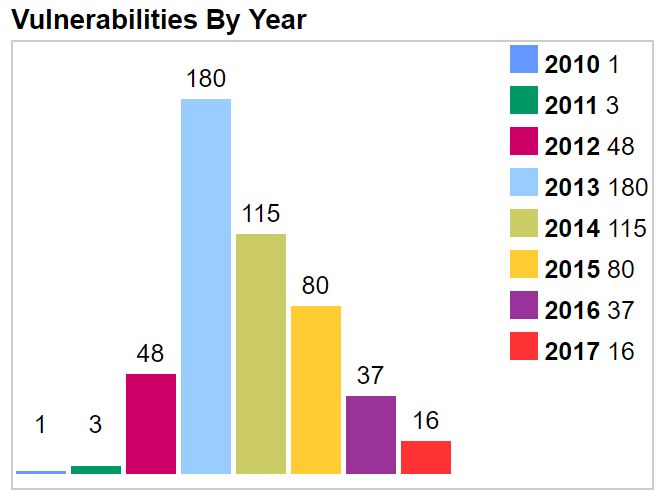
\includegraphics[scale=0.25]{content/images/cvedetails_vulnsperyear.png}
			\caption{Total CVEs by year \cite{cvedetails:jdk2016}}
		\end{figure}
	\end{columns}	
\end{frame}

\begin{frame}{Writing Secure Java Code}
	Developers of security conscious Java applications must ensure the Confidentiality, Integrity and Availability of data. They can do this by:
	
	\begin{itemize}
		\item Following the Oracle Secure Coding Guidelines
		\item Running their application with a \texttt{SecurityManager} installed
		\item Following the Principle of Least Privilege
	\end{itemize}
	
	What they usually can't do is \textit{prove it}.
\end{frame}

\begin{frame}{Thesis Topic}
	One avenue for providing \textit{provable} Confidentiality and Integrity to programs is applying the theory of \textit{Information Flow}.
	
	This leads to the key question this thesis aims to address:
	
	\begin{block}{Key Thesis Question}
		Can Information Flow be used to provide practical improvements to the Confidentiality and Integrity of Java programs?
	\end{block}
\end{frame}

\begin{frame}{Thesis Overview}
	\begin{block}{Key Thesis Question}
		Can Information Flow be used to provide practical improvements to the Confidentiality and Integrity of Java programs?
	\end{block}

	To answer this question, this thesis aims to evaluate both the relevance of information flow-based security, and current implementations of it, to determine:
	
	\begin{enumerate}
		\item What practical security benefits Information Flow can provide
		\item Whether Information Flow is viable for real world applications
	\end{enumerate}
\end{frame}